% =============================================================================
% DiD-BCF revision: small panels, the pre-trend diagnostic, and the
% already-treated contamination ramp.
% Companion to revision_simulation_report.tex; shares its tables/ and figures/.
% =============================================================================
\documentclass[11pt]{article}

\usepackage[a4paper,margin=2.5cm]{geometry}
\usepackage{amsmath,amssymb,mathtools}
\usepackage{booktabs}
\usepackage{array}
\usepackage{longtable}
\usepackage{graphicx}
\usepackage{microtype}
\usepackage[hidelinks]{hyperref}

\newcommand{\att}{\mathrm{ATT}}
\newcommand{\gatt}{\mathrm{GATT}}
\newcommand{\es}{\mathrm{ES}}
\newcommand{\catt}{\mathrm{CATT}}
\newcommand{\ind}{\mathbb{1}}

\graphicspath{{figures/}}

\title{\textbf{Forests for Differences}: small panels, the pre-trend
diagnostic, and already-treated contamination}
\author{Simulation report, second interim instalment}
\date{20 August 2026}

\begin{document}
\maketitle

\begin{abstract}
This report covers the three parts of the revision grid that the first interim
report could not: the small-panel end of the B2 sample-size sweeps at $N=50$
and $N=100$, the operating characteristics of the proposed pre-trend
diagnostic on the ten \texttt{PT\_*} designs, and the behaviour of every
estimator in the suite as the Goodman--Bacon weight on already-treated
comparisons is raised from $0.077$ to $0.250$ on the \texttt{D\_ramp\_*}
designs. It also documents three data-integrity corrections applied to the
aggregation layer before any number below was computed.

The small-panel results are favourable to the plain structured DiD-BCF fit on
point estimation and unfavourable to it on inference. At $N=50$ its pooled
$\att$ RMSE is $0.237$ in the ordinary sweep, against $0.363$ for synthetic
DiD and $0.459$ for the posterior-corrected fit, and its individual-level CATT
surface RMSE is $0.452$ against $1.09$ to $1.31$ for every cohort-time method;
but its posterior spread is only $0.54$ to $0.70$ of the Monte-Carlo error
dispersion, and in the serial sweep its $\att$ coverage sits at $0.83$ at every
panel size. The posterior correction repairs exactly that: its calibration
ratio is close to one at every size and its coverage is at or above nominal
throughout, at a roughly doubled RMSE. Callaway--Sant'Anna is the only
estimator that fails to return an estimate at $N=50$, losing four replications
in a hundred at $d=2$ and $d=3$.

The pre-trend diagnostic is correctly sized ($0.045$ against a nominal $0.05$
when conditional parallel trends holds) and dominates the standard-practice
TWFE event-study placebo in power at every violation magnitude, most sharply at
the smallest one, where it detects $0.220$ against $0.100$. It is also the only
pre-test in the comparison that stays quiet when conditional parallel trends
holds but unconditional parallel trends fails, rejecting $0.080$ where the
marginal event study and Gardner's two-stage pre-test reject about $0.75$. The
power advantage over Callaway--Sant'Anna's and grf-DiD's own conditional
pre-tests is real but much smaller, so the honest claim is that the diagnostic
matches the best available conditional pre-test and beats the marginal one, not
that it is unique.

The contamination ramp gives the clearest negative result in the suite. TWFE's
pooled $\att$ bias rises from $0.261$ to $1.181$ and its coverage falls from
$0.885$ to $0.000$ across the weight axis, as intended. But DiD-BCF also
degrades, from $0.003$ to $0.247$ (plain) and $0.007$ to $0.149$ (corrected),
while Callaway--Sant'Anna, Gardner and grf-DiD stay flat near $0.01$ to $0.03$.
DiD-BCF is therefore much more robust than TWFE to already-treated
contamination and clearly less robust than the estimators built to eliminate
it.
\end{abstract}

\tableofcontents

% =============================================================================
\section{Scope and what is new}
% =============================================================================

The first interim report analysed the complete structured grid over the B1,
B2 and D designs at panel sizes $N\in\{200,400,800,1600\}$. Three things have
changed since, and this report is confined to them.

First, the sample-size sweep was redefined. The live grid is
$N\in\{50,100,200,400,800\}$: the $N=1600$ column was dropped and two smaller
panels were added below the base size, so the sweep now brackets the base
panel of $200$ on both sides instead of only extending above it. The two new
columns were produced locally rather than on Colab, because at these sizes
none of the five benchmark estimators is slow.

Second, the ten \texttt{PT\_*} designs have completed at $200$ replications
and at linearity degrees $d=1$ and $d=3$, for the DiD-BCF diagnostic and for
the pre-tests native to Callaway--Sant'Anna, Gardner, synthetic DiD, grf-DiD
and DoubleML, plus a TWFE event-study placebo run on the same replications.
The first report contained a $24$-replication fragment of three of these
designs at $d=1$ only.

Third, the six \texttt{D\_ramp\_nt*} designs have completed at $200$
replications for every estimator, so estimator error can now be plotted
against a measured Goodman--Bacon weight rather than against a design knob
that does not move that weight.

Section~\ref{sec:integrity} documents corrections made to the aggregation
layer before any number in this report was computed; readers comparing against
earlier drafts should read it first, because two of the three corrections
change published figures.

% =============================================================================
\section{Data-integrity corrections applied in this pass}
\label{sec:integrity}
% =============================================================================

Three defects in the result-collection layer were found and fixed. All numbers
in this report were computed after the fixes.

\paragraph{The sample-size label on three benchmark estimators.} The
Callaway--Sant'Anna, Gardner and synthetic-DiD summary files for the sweep
panels at $N\in\{400,800,1600\}$ carried the value $200$ in their \texttt{N}
column. The panels themselves were correct, with $400$, $800$ and $1600$
distinct units respectively; only the recorded label was wrong, a residue of
an older version of the R driver that hard-coded the base size instead of
reading it off the data. Because the aggregation layer de-duplicates on the
key (setting, degree, $N$, replication, estimand, method), the mislabelled
rows collided with the genuine $N=200$ rows and were silently discarded. The
consequence was that these three estimators appeared in the aggregated tables
at $N=200$ only, and the first report's statement that the sweep was complete
for them was therefore incorrect. The current R drivers compute $N$ from the
panel, so the affected cells were simply re-run; all twelve re-runs completed.

\paragraph{The pre-trend results were not being collected.} The aggregation
layer globbed \url{Results/summaries_pretrend_*.csv}, which holds a
$24$-replication fragment of three designs at $d=1$, but not
\url{Pretrend/summaries_pretrend_*.csv}, which holds the completed
$200$-replication runs of all ten designs at $d=1$ and $d=3$. Every pre-trend
number in the first draft was therefore computed on roughly one eighth of the
available replications. The two sources were verified to agree exactly on
their $888$ overlapping rows before the second was added, so the correction
adds replications without revising any completed one.

\paragraph{The sweep axis was hard-coded in the figure code.} Three figure
routines drew tick marks at $200$, $400$, $800$ and $1600$ regardless of the
configured sweep, so the two new panels would have been plotted outside the
visible axis. The axis is now read from the configuration.

One further gap is documented rather than fixed. The DiD-BCF fits for the two
middle ramp designs, \texttt{D\_ramp\_nt20} and \texttt{D\_ramp\_nt25},
have not been run: the notebooks exist but no summary files do. Every ramp
result below therefore shows DiD-BCF at four of the six weights, at
$0.077$, $0.100$, $0.196$ and $0.250$, and the two interior points are dashes
rather than interpolations. The competitor estimators and TWFE are present at
all six.

% =============================================================================
\section{Designs}
% =============================================================================

\subsection{The small-panel extension of B2}

The two B2 sweeps are unchanged in every respect except the panel size. The
ordinary sweep is the canonical two-period-block design with independent
idiosyncratic errors; the serial sweep is the same design with an $AR(1)$
coefficient of $0.6$ on the within-unit error. Both are generated at
$N\in\{50,100,200,400,800\}$ and at linearity degrees $d\in\{1,2,3\}$, with
$100$ replications per cell, four pre-periods and four post-periods. The
replications are seeded by index, so the panel handed to the R estimators is
byte-identical to the one the DiD-BCF notebooks regenerate in memory, and the
comparison at a given $(N,d,\text{replication})$ is a comparison of estimators
on one dataset rather than of estimators on independent draws.

At $N=50$ the design has $50$ units observed over $8$ periods, of which
roughly half are treated from period $5$: the cohort-time cell
$\gatt(4,4)$ is therefore estimated from on the order of twenty-five treated
units, which is the regime in which a forest-based prior does most of its work
and in which a doubly-robust estimator has the least room to cross-fit.

\subsection{The pre-trend designs}

Ten canonical designs isolate one question each. \texttt{PT\_hold} is the
baseline design, in which conditional parallel trends holds and every
rejection is a false positive, so it measures size. The four
\texttt{PT\_violation\_g*} designs put the treated group on a differential
linear path of slope $0.05$, $0.10$, $0.20$ and $0.40$ outcome units per
period, tracing a power curve against violation magnitude.
\texttt{PT\_violation\_a20} routes a violation of the same nominal magnitude
through the \emph{unobserved} confounder rather than through the group
indicator, which no adjustment on observables can remove; the realised slope
is $0.207$, close by construction to the $0.20$ of the matching group-trend
design. The three \texttt{PT\_violation\_het*} designs impose a differential
slope of $\pm\kappa$ that depends on the observed covariate $X_1$ and cancels
in the aggregate, with $\kappa\in\{0.10,0.20,0.40\}$: the realised aggregate
slope is zero to three decimals, so an aggregate pre-test is powerless there
by construction and only a subgroup contrast can see the violation. Finally
\texttt{PT\_conditional} is the discrimination case, in which conditional
parallel trends holds while unconditional parallel trends fails, because
assignment depends on a covariate that also shifts trends. A diagnostic whose
job is to test the assumption the estimator actually makes should stay quiet
there; a marginal event study, which does not condition, should not.

Each design is run at $200$ replications at $N=200$ and at degrees $d=1$ and
$d=3$. Two decision rules are reported. The \emph{slope} rule tests the single
differential-trend coefficient implied by the estimated pre-period path
$\Delta(k)$; the \emph{any-$k$} rule flags if any individual pre-period
$\Delta(k)$ is significant after a Bonferroni scaling. When the violation is a
linear differential trend the slope rule is the efficient one, so it is
reported as the headline and the any-$k$ rule as the conservative alternative.

\subsection{The already-treated contamination ramp}

The original ramp swept the \texttt{dynamic\_ramp} parameter, which changes how
\emph{inconsistent} the already-treated comparisons are but leaves their
Goodman--Bacon \emph{weight} exactly constant at $0.116$, because that weight
is a function of the adoption design alone. It therefore could not support any
claim about what happens as already-treated comparison weight rises. The
current design sweeps the never-treated share instead, over
$\{0.40,0.30,0.25,0.20,0.10,0.05\}$, holding the effect DGP fixed. Shrinking
the clean control pool moves the measured mean weight on ``later versus
earlier'' comparisons from $0.077$ to $0.250$, and that measured weight is the
$x$-axis of every result in Section~\ref{sec:ramp}. Each design is a staggered
three-cohort adoption with cohort effect multipliers $(1.0,1.5,2.0)$ and a
dynamic ramp of $0.4$, at $N=200$ with $200$ replications and $d\in\{1,2,3\}$.

Because the estimators report different estimands natively, the ramp results
are read in three internally consistent panels: a pooled $\att$ for DiD-BCF,
TWFE and synthetic DiD; cohort-time cells for Callaway--Sant'Anna, DoubleML
and grf-DiD; and event-study coefficients for Gardner. No estimator is scored
on a target it does not estimate.

% =============================================================================
\section{Small panels: $N=50$ and $N=100$}
% =============================================================================

\subsection{Point estimation}

Table~\ref{tab:smalln} reports the cohort-time target $\gatt(4,4)$ and the
pooled $\att$ at $N\in\{50,100,200\}$ and $d=1$, with $N=200$ carried as the
reference column because it is the base panel of every other scenario in the
suite. Figure~\ref{fig:smalln} extends the same quantities across the whole
sweep.

Every estimator has small bias at every panel size: the largest absolute
$\gatt(4,4)$ bias anywhere in the $d=1$ small-panel block is $0.083$, for the
corrected fit at $N=50$, and most entries are an order of magnitude below the
corresponding RMSE. The small-sample problem in this design is therefore
dispersion, not location.

On dispersion the plain structured fit wins, and not narrowly. At $N=50$ in
the ordinary sweep its $\gatt(4,4)$ RMSE is $0.250$, against $0.409$ for
grf-DiD, $0.455$ for Callaway--Sant'Anna, $0.707$ for the corrected fit and
$0.729$ for DoubleML. At $N=100$ the ordering is unchanged, at $0.168$ against
$0.298$, $0.290$, $0.342$ and $0.467$. The same holds on the pooled $\att$,
where at $N=50$ the plain fit's RMSE of $0.237$ compares with $0.363$ for
synthetic DiD and $0.459$ for the corrected fit. The advantage narrows as $N$
grows but does not vanish: at $N=800$ the plain $\att$ RMSE is $0.051$ against
$0.092$ for synthetic DiD. This is the expected behaviour of a strong
regularising prior in a small sample, and it is the clearest quantitative
argument in the suite for the DiD-BCF approach at panel sizes typical of
applied work.

\input{tables/tab_smalln.tex}

\begin{figure}[htbp]
\centering
\includegraphics[width=0.98\linewidth]{fig_smalln.pdf}
\caption{Pooled $\att$ RMSE, pooled $\att$ coverage, and individual-level
CATT-surface RMSE across the full B2 ordinary sweep at $d=1$. The two smallest
panels are the new columns.}
\label{fig:smalln}
\end{figure}

\subsection{Inference, and the price of the prior}

The same prior that buys the point-estimation advantage is paid for in the
interval. The calibration ratio $\overline{\mathrm{sd}}/\mathrm{SD}$, the mean
reported posterior spread divided by the Monte-Carlo standard deviation of the
error, is the diagnostic: a value below one means the estimator is reporting
less uncertainty than it actually has. For the plain fit it is $0.70$ at
$N=50$ and $0.84$ at $N=200$ on the ordinary-sweep $\att$, and $0.54$, $0.58$
and $0.60$ at $N=50$, $100$ and $200$ on the serial-sweep $\att$. The serial
figures do not improve with $N$ at all, which is what one expects of a
specification that does not model the within-unit dependence: the shortfall is
a missing variance component, not a small-sample artefact. Coverage follows:
the plain serial $\att$ covers $0.83$, $0.80$, $0.83$, $0.85$ and $0.83$ at
the five panel sizes, flat and roughly twelve points below nominal.

The posterior correction repairs precisely this. Its calibration ratio on the
serial $\att$ is $0.96$, $1.17$, $1.10$, $1.09$ and $0.92$ across the sweep and
its coverage is $0.97$ or above at every size, at the cost of an RMSE roughly
$1.1$ to $1.3$ times the plain fit's on that target, and about twice the plain
fit's on the ordinary sweep. At $d=1$ this is a clean
efficiency-for-honesty trade and the correction is the specification to report
when interval coverage matters.

That endorsement does not survive the nonlinear degrees at small $N$. At
$d=2$ and $N=50$ the corrected ordinary-sweep $\gatt(4,4)$ RMSE is $2.517$,
ten times the plain fit's $0.263$ and five times Callaway--Sant'Anna's
$0.462$; at $d=3$ it is $2.455$. The instability persists into the middle of
the sweep, with a corrected RMSE of $1.319$ at $N=400$ and $d=2$ against
$0.092$ for the plain fit, before recovering to $0.318$ at $N=800$. Coverage
stays near nominal throughout, so the correction is not producing confidently
wrong answers; it is producing very wide ones. The practical reading is that
the cross-fitted correction needs either a larger panel or a degree-one
nuisance structure to be stable, and that the corrected estimator should not
be presented as a general-purpose replacement for the plain fit.

\subsection{Estimability at $N=50$}

Callaway--Sant'Anna is the only estimator in the comparison that fails to
return an estimate. At $N=50$ and degrees $d=2$ and $d=3$ it returns nothing
for any cohort-time cell in four replications out of a hundred in both sweeps,
so its retention is $0.96$; at $N=100$ it is $0.99$ and at $N\geq200$ it is
$1.00$. DoubleML loses one replication at $N=50$ in the serial sweep at $d=1$ and
two at $d=3$. Every other estimator, including both DiD-BCF
specifications, returns an estimate in every replication at every cell. The
metrics layer computes all statistics on the replications that produced an
estimate and records the retained fraction alongside, so the affected cells
are marked in Table~\ref{tab:smalln} rather than being silently averaged; a
coverage of $0.94$ over $96$ replications is not the same statement as a
coverage of $0.94$ over $100$, and the distinction matters most at exactly the
panel size where the comparison is being made.

\subsection{The CATT surface}

Table~\ref{tab:smallnsurface} reports the individual-level surface: the
within-replication RMSE, MAPE and pointwise coverage over the treated
observations. Every estimator other than DiD-BCF reports a single number per
cohort-time cell, so its surface is that number broadcast to the individuals
in the cell, and the comparison measures exactly what is lost by not modelling
individual heterogeneity.

The result is the strongest in this report. At $N=50$ in the ordinary sweep
the plain fit's surface RMSE is $0.452$ with a MAPE of $0.113$ and pointwise
coverage of $0.92$; every cohort-time method sits between $1.09$ and $1.31$
with a MAPE near $0.28$ and coverage between $0.50$ and $0.75$. The gap is
present at the smallest panel in the grid, which is the most demanding place
to claim it, and it widens with $N$ rather than closing: at $N=800$ the plain
surface RMSE is $0.155$ against $1.06$ for the cohort-time methods, whose
surface error is bounded below by the within-cell heterogeneity they cannot
represent and therefore does not converge. grf-DiD is the only benchmark that
improves along this axis, from $1.155$ at $N=50$ to $0.367$ at $N=800$,
because it also produces individual-level predictions; it remains between two and three times the plain fit's error at every
size.

Two qualifications belong with that result. The corrected fit does not share
it: its surface RMSE is $1.209$ at $N=50$ and $1.064$ at $N=800$, in the
cohort-time band rather than the DiD-BCF band, because the correction
recentres the posterior at the cell level and discards the individual
variation. And the plain fit's surface advantage coexists with its
scalar-interval shortfall documented above, so the honest summary is that the
plain specification is the one to use for heterogeneity and the corrected one
for pooled inference.

\input{tables/tab_smalln_surface.tex}

% =============================================================================
\section{The pre-trend diagnostic}
% =============================================================================

\subsection{Size, power and discrimination}

Table~\ref{tab:pretrend} reports the diagnostic against the TWFE event-study
placebo at $d=1$; Table~\ref{tab:pretrendd3} repeats it at $d=3$. All figures
are over $200$ replications, except \texttt{PT\_violation\_het20} at $d=3$,
where one block of $50$ replications is missing and the figures are over $150$.

Under \texttt{PT\_hold} the diagnostic rejects $0.045$ of the time against a
nominal $0.05$, with a Monte-Carlo standard error of about $0.015$, and the
any-$k$ rule rejects $0.030$. At $d=3$ the corresponding figures are $0.055$
and $0.045$. The diagnostic is correctly sized, and the conservative rule is
conservative as intended.

Power rises monotonically with the violation, from $0.220$ at a slope of
$0.05$ through $0.520$ at $0.10$ and $0.935$ at $0.20$ to $1.000$ at $0.40$.
The TWFE event-study placebo run on the same replications rejects $0.100$,
$0.250$, $0.700$ and $1.000$. The advantage is therefore largest where it
matters most, at the small violations that a pre-test is actually needed to
catch: at a slope of $0.05$ the diagnostic more than doubles the placebo's
rejection rate, and at $0.10$ it roughly doubles it, while at $0.40$ both
detect everything. The violation routed through the unobserved confounder
behaves like the group-trend violation of the same realised magnitude, at
$0.930$ against $0.705$, confirming that the diagnostic responds to the
differential path rather than to the channel that produced it.

Discrimination is the sharpest of the three results. Under
\texttt{PT\_conditional}, where the estimator's own assumption is satisfied
and only unconditional parallel trends fails, the diagnostic rejects $0.080$
while the marginal event study rejects $0.755$. Standard practice would
reject a correctly specified analysis in three cases out of four here. The
diagnostic's slope estimate is also nearly unbiased in that design, at $0.055$
against a true zero with $0.950$ coverage, whereas the event study's slope
carries a bias of $0.287$ and covers $0.245$.

\begin{table}[htbp]
\centering
\footnotesize
\caption{Operating characteristics of the pre-trend diagnostic at $d=1$,
against the TWFE event-study placebo run on the same replications. 200
replications per scenario.}
\label{tab:pretrend}
\input{tables/tab_pretrend.tex}
\end{table}

\begin{figure}[htbp]
\centering
\includegraphics[width=0.98\linewidth]{fig_pretrend.pdf}
\caption{Detection rate against the realised differential pre-trend slope, the
estimated $\Delta(k)$ profiles, and the ATT bias the violation induces, at
$d=1$.}
\label{fig:pretrend}
\end{figure}

\subsection{Against the benchmarks' own pre-tests}

Comparing the diagnostic only against a marginal event study overstates the
case, because Callaway--Sant'Anna, grf-DiD, Gardner, DoubleML and synthetic
DiD all admit pre-tests of their own and three of them condition on
covariates. The full comparison is in \url{Pretrend/BENCHMARK_TABLES.txt} and
its qualitative content is as follows.

On the group-trend power curve at $d=1$ the diagnostic leads, at $0.220$,
$0.520$, $0.935$ and $1.000$, against $0.090$, $0.320$, $0.830$ and $1.000$
for Callaway--Sant'Anna, $0.085$, $0.285$, $0.795$ and $1.000$ for grf-DiD,
$0.095$, $0.240$, $0.700$ and $1.000$ for Gardner, and $0.085$, $0.180$,
$0.540$ and $0.985$ for DoubleML. The margin over the best conditional
competitor is therefore about thirteen points at the smallest violation and
twenty at the second smallest, which is a real but modest advantage, not the
order-of-magnitude gap the comparison against the marginal event study
suggests. Synthetic DiD is a special case: its pre-test rejects $0.000$ at slopes up
to $0.10$ and only $0.170$ at $0.20$, because the synthetic-control weights
absorb the differential trend into the fit, so it is barely a pre-test of the
assumption at all.

Two competitors fail the discrimination case in the same way the marginal
event study does. Gardner rejects $0.750$ and the TWFE placebo $0.755$ under
\texttt{PT\_conditional}, because both pre-test an unconditional path;
Callaway--Sant'Anna rejects $0.070$ and grf-DiD $0.100$, close to the
diagnostic's $0.080$. The defensible claim is therefore narrower than
``uniquely able to discriminate'': the diagnostic, Callaway--Sant'Anna's
pre-test and grf-DiD's pre-test all correctly stay quiet, and the two
unconditional pre-tests do not.

\subsection{The heterogeneous violation}

The three \texttt{PT\_violation\_het*} designs impose a violation that cancels
in the aggregate, so the realised aggregate slope is zero to three decimals.
Every aggregate pre-test correctly rejects at about its nominal rate there,
between $0.040$ and $0.115$; that is the right answer, not a failure, and the
induced ATT bias confirms it, at $-0.005$ to $-0.001$ for the plain fit. The
interesting quantity is the subgroup contrast in $X_1$, which is the only
statistic that can see this violation. The realised contrast slope is $2\kappa$. At a contrast slope of $0.40$ the
diagnostic's contrast rejects $0.520$, Callaway--Sant'Anna's $0.745$,
grf-DiD's $0.700$ and Gardner's $0.665$; at $0.80$ all four reach $1.000$; at
$0.20$ the diagnostic rejects $0.020$ against $0.320$, $0.275$ and $0.235$. On this
axis the diagnostic is the least powerful of the four conditional pre-tests,
not the most, and its contrast slope is materially biased, at $-0.111$ to
$-0.141$ against true values of $0.20$ to $0.80$, whereas
Callaway--Sant'Anna's contrast is unbiased to three decimals. The subgroup
contrast should therefore be reported as a diagnostic that exists rather than
as one that outperforms; the aggregate slope rule is where the DiD-BCF
diagnostic is strong.

\subsection{Tying detection to consequence}

Panel (c) of Figure~\ref{fig:pretrend}, tabulated in
\url{Results/aggregated/pretrend_all.csv}, reports the ATT bias the violation
actually induces, which is what a pre-test is ultimately protecting against.
At a slope of $0.05$ the plain fit's ATT bias is $0.194$ and the diagnostic
detects the violation in $0.220$ of replications; at $0.10$ the bias is
$0.393$ and detection is $0.520$; at $0.20$, $0.787$ and $0.935$; at $0.40$,
$1.575$ and $1.000$. Detection therefore lags consequence at the low end, and
the honest statement is that a violation large enough to bias the ATT by about
a fifth of a unit will be missed four times in five by the marginal event
study and about four times in five by the diagnostic as well. The posterior
correction halves the induced bias throughout, at $0.109$, $0.230$, $0.474$
and $0.960$ against the plain fit's figures, which is a further argument for
the correction in designs where a residual violation is plausible.

\begin{figure}[htbp]
\centering
\includegraphics[width=0.98\linewidth]{fig_pretrend_d3.pdf}
\caption{The same three panels at linearity degree $d=3$. The nonlinear
nuisance axis leaves the diagnostic's size, power and discrimination
essentially unchanged.}
\label{fig:pretrendd3}
\end{figure}

\begin{table}[htbp]
\centering
\footnotesize
\caption{The same operating characteristics at $d=3$.
\texttt{PT\_violation\_het20} is over 150 replications; every other row is over
200.}
\label{tab:pretrendd3}
\input{tables/tab_pretrend_d3.tex}
\end{table}

The degree axis does not disturb any of this. At $d=3$ size is $0.055$, the
power curve reads $0.230$, $0.510$, $0.900$ and $1.000$, and discrimination is
$0.100$ against the event study's $0.755$. Every figure is within Monte-Carlo
error of its $d=1$ counterpart, which is a useful robustness statement given
how sensitive the corrected ATT estimator is to the same axis.

% =============================================================================
\section{Already-treated contamination}
\label{sec:ramp}
% =============================================================================

\subsection{What the ramp shows}

Table~\ref{tab:rampmethods} and Figure~\ref{fig:rampmethods} report mean
absolute error and coverage against the measured Goodman--Bacon weight on
already-treated comparisons, in the three estimand panels described above.

TWFE behaves exactly as the Goodman--Bacon decomposition predicts. Its pooled
$\att$ absolute bias rises monotonically from $0.261$ at a weight of $0.077$
through $0.468$ at $0.116$ to $1.181$ at $0.250$, and its coverage collapses
from $0.885$ to $0.690$, $0.500$, $0.240$, $0.005$ and $0.000$. On the
event-study panel the same pattern is stronger still, from $0.183$ to $1.383$
with coverage from $0.970$ to $0.238$. Against a true pooled effect of about
$5.3$ the largest bias is roughly $22$ percent. This is the reviewer's
question answered directly and it fully justifies excluding pooled TWFE as the
headline benchmark for heterogeneous staggered designs.

Synthetic DiD is a different failure. Its pooled $\att$ absolute bias is
$1.247$ at the lowest weight and $1.314$ at the highest, essentially flat, with
coverage of $0.000$ almost throughout. The error is not contamination; the
estimator is targeting the weighted estimand its own weights define, which in
a design with cohort effect multipliers $(1.0,1.5,2.0)$ is not the equally
weighted $\att$ used as the truth here. It should be read as an estimand
mismatch and not cited as evidence about already-treated comparisons.

The three estimators built to eliminate the contamination do so. On the
cohort-time panel Callaway--Sant'Anna's mean absolute error runs $0.013$,
$0.014$, $0.012$, $0.017$, $0.017$, $0.033$ and grf-DiD's runs $0.021$,
$0.021$, $0.022$, $0.028$, $0.012$, $0.016$; on the event-study panel
Gardner's runs $0.010$ to $0.008$. All three are flat in the weight, as they
should be, since none uses an already-treated unit as a control. DoubleML is
the exception among the covariate-adaptive benchmarks: its error rises from
$0.023$ to $0.200$ over the axis, which is a real degradation, though an order
of magnitude smaller than TWFE's.

\subsection{Where DiD-BCF stands}

DiD-BCF is much better than TWFE and clearly worse than the purpose-built
estimators. Its pooled $\att$ absolute bias rises from $0.003$ to $0.247$
(plain) and from $0.007$ to $0.149$ (corrected) across the four weights at
which it was run, against TWFE's $0.261$ to $1.181$ over the same span. At the highest weight the plain fit's pooled error is a fifth of TWFE's on
the same panel; the purpose-built estimators sit near $0.03$ on their own
panels, an order of magnitude below it, though that last comparison crosses
estimands and should be read as indicative. Coverage tells the same story more sharply: the
plain fit's pooled $\att$ coverage falls from $0.975$ to $0.850$ and $0.670$,
while the corrected fit holds $0.975$ or above at every weight. This is the
second design family, after the serial sweep, in which the correction is doing
real inferential work.

Two further observations belong in the write-up. First, on the cohort-time
panel the plain fit's mean absolute error is roughly $0.25$ at \emph{every}
weight, including the lowest, with coverage near $0.73$. That is not
contamination; it is the flat, weight-independent cell-level recentring
already documented for the plain specification, and the ramp is not the place
to diagnose it. The corrected fit removes it at low weight, at $0.024$, and
loses it again at high weight, at $0.339$. Second, the corrected fit is
unstable on this design family at the nonlinear degrees, with a pooled $\att$
error of $0.384$ at a weight of $0.100$ and $d=2$ against $0.050$ at $0.077$,
which is the same instability seen at small $N$ in Section~4 and points to the
cross-fitted pilot rather than to the design.

\begin{table}[htbp]
\centering
\footnotesize
\caption{Mean absolute error against the measured Goodman--Bacon weight on
already-treated comparisons, by natively reported estimand, at $d=1$. 200
replications per design.}
\label{tab:rampmethods}
\begin{tabular}{llrrrrrr}
\toprule
& & \multicolumn{6}{c}{Weight on already-treated comparisons} \\
\cmidrule(lr){3-8}
Estimand & Estimator & 0.077 & 0.100 & 0.116 & 0.136 & 0.196 & 0.250 \\
\midrule
ATT & DiD-BCF (plain) & 0.003 & 0.015 & -- & -- & 0.119 & 0.247 \\
 & DiD-BCF (corrected) & 0.007 & 0.014 & -- & -- & 0.044 & 0.149 \\
 & TWFE & 0.261 & 0.386 & 0.468 & 0.573 & 0.889 & 1.181 \\
 & Synthetic DiD & 1.247 & 1.269 & 1.280 & 1.290 & 1.300 & 1.314 \\
\midrule
GATT & DiD-BCF (plain) & 0.251 & 0.253 & -- & -- & 0.294 & 0.357 \\
 & DiD-BCF (corrected) & 0.024 & 0.035 & -- & -- & 0.113 & 0.339 \\
 & Callaway--Sant'Anna & 0.013 & 0.014 & 0.012 & 0.017 & 0.017 & 0.033$^{\dagger}$ \\
 & DoubleML DR-DiD & 0.023 & 0.023 & 0.017 & 0.021 & 0.086 & 0.200$^{\dagger}$ \\
 & grf-DiD (Wang) & 0.021 & 0.021 & 0.022 & 0.028 & 0.012 & 0.016 \\
\midrule
ES & DiD-BCF (plain) & 0.100 & 0.113 & -- & -- & 0.242 & 0.379 \\
 & DiD-BCF (corrected) & 0.011 & 0.012 & -- & -- & 0.076 & 0.258 \\
 & TWFE & 0.183 & 0.309 & 0.396 & 0.507 & 0.881 & 1.383 \\
 & Gardner (did2s) & 0.010 & 0.013 & 0.012 & 0.009 & 0.006 & 0.008 \\
\bottomrule
\end{tabular}
\par\smallskip\footnotesize $^{\dagger}$Computed on the replications in which the estimator returned an estimate: Callaway--Sant'Anna retains 92\% of replications at this design, so the figure is a selected subsample and is not comparable with estimators that ran everywhere.

\end{table}

\begin{figure}[htbp]
\centering
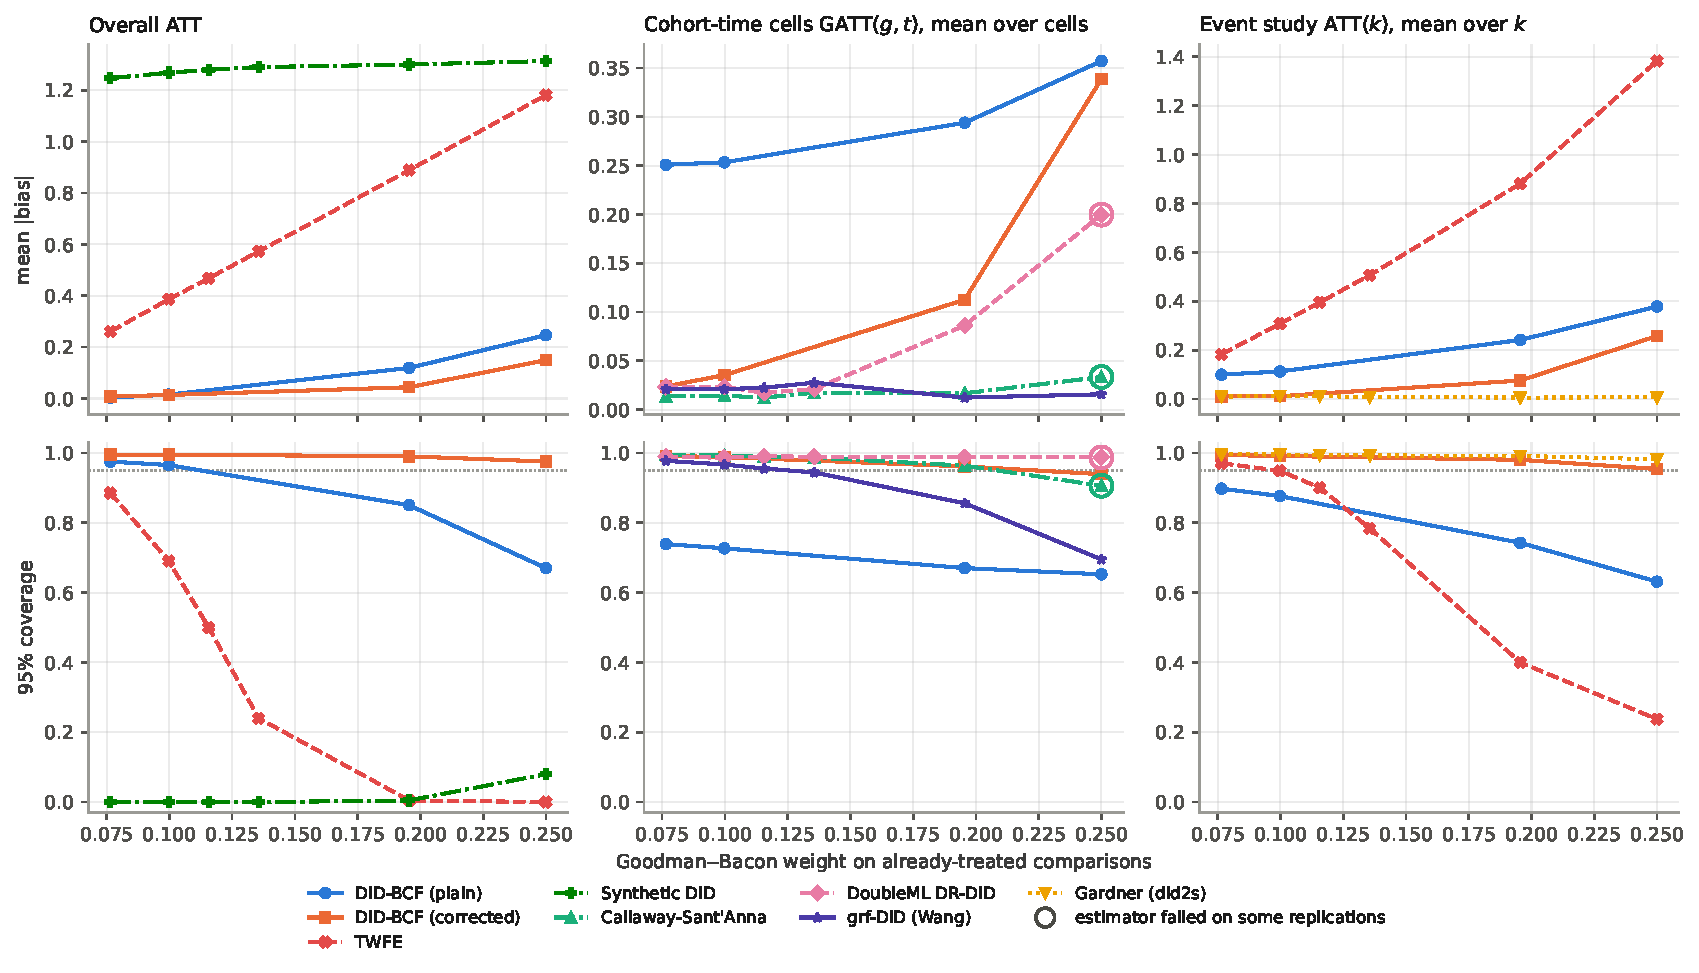
\includegraphics[width=0.98\linewidth]{fig_ramp_methods.pdf}
\caption{Mean absolute error and 95\% coverage against the measured
Goodman--Bacon weight on already-treated comparisons, by natively reported
estimand, at $d=1$.}
\label{fig:rampmethods}
\end{figure}

\subsection{Estimability along the ramp}

Callaway--Sant'Anna's estimability degrades along this axis, from a retention
of $1.00$ at the lowest weight to $0.92$ at the highest at $d=1$, and to
$0.785$ at $d=2$ and $d=3$. DoubleML retains $0.925$ at the highest weight.
The two cells so affected are marked in Table~\ref{tab:rampmethods}, because a
mean error computed on the $78.5$ percent of replications in which the
estimator converged is a selected subsample and is not comparable with an
estimator that ran everywhere. That the flattest error curve in the table
belongs to the estimator with the highest failure rate at the hardest design
is itself worth stating.

% =============================================================================
\section{Interpretation and remaining work}
% =============================================================================

Three claims are now supported by completed evidence and can go into the
revision as they stand. The first is that the plain structured DiD-BCF fit
dominates every benchmark on individual-level heterogeneity recovery at every
panel size in the sweep, including $N=50$, by a factor of two against the best
benchmark and a factor of five or more against every cohort-time method. The
second is that the proposed pre-trend diagnostic is correctly sized, more
powerful than the standard-practice marginal event-study placebo at every
violation magnitude, and correctly quiet in the design where conditional
parallel trends holds but unconditional parallel trends does not. The third is
that pooled TWFE is unusable as a benchmark in staggered designs with a small
never-treated pool, with bias up to $22$ percent of the true effect and
coverage of zero.

Three claims are not supported and should not be made. Pre-trend
discrimination is not unique to the diagnostic: Callaway--Sant'Anna's and
grf-DiD's conditional pre-tests do the same job, and the diagnostic's
advantage over them on the power curve is on the order of fifteen points, not
an order of magnitude. The subgroup contrast is the weakest of the four
conditional pre-tests on the heterogeneous-violation designs and its contrast
slope is biased, so it should be presented as available rather than as
superior. And DiD-BCF is not robust to already-treated contamination in the
way Callaway--Sant'Anna, Gardner and grf-DiD are: its error grows by two
orders of magnitude across the weight axis, from $0.003$ to $0.247$, even
though it stays far below TWFE throughout.

The posterior correction now has a consistent profile across three design
families. It repairs the plain fit's interval calibration wherever that
calibration is broken, which is the serial sweep at every $N$, the small
panels, and the high-contamination end of the ramp, and it does so at roughly
double the RMSE. It is unstable at the nonlinear degrees whenever the
effective sample is small, at $N\leq400$ in the sweeps and at the interior
weights of the ramp, and it discards the individual-level heterogeneity that
is the plain fit's main advantage. The recommendation that follows is to
report both specifications side by side rather than to choose, with the plain
fit carrying the heterogeneity results and the corrected fit carrying the
pooled inference.

Four gaps remain. The DiD-BCF fits for \texttt{D\_ramp\_nt20} and
\texttt{D\_ramp\_nt25} have not been run, so the ramp shows DiD-BCF at four of
six weights. One block of fifty replications is missing from
\texttt{PT\_violation\_het20} at $d=3$. The \texttt{PT\_*} designs carry
DiD-BCF ATT results at $d=1$ only, so the detection-versus-consequence
comparison of Section~5.5 has no $d=3$ counterpart. And TWFE was not run on the sweeps
below $N=200$, so it is absent from the two smallest columns of
Table~\ref{tab:smalln}.

\end{document}
